\documentclass[12pt,openright,twoside,french]{book}

\input philippe2013
\input philippe2013_activites
\pagestyle{empty}


\begin{document}

\TitreActivite{x.1}{Loi binomiale et \par \'Echantillonnage}

\begin{minipage}{0.6\linewidth}
Soit $X$ la variable aléatoire qui suit la loi binomiale de paramètres $(30 \pv 0,3)$.\par
On détermine, avec un tableur, la table de probabilité et la table de probabilité cumulée croissante de cette loi.

\begin{enumerate}
    \item À l'aide de la cette table, déterminer les probabilités suivantes, arrondies à $\np{0,00001}$ près :
        \begin{enumerate}
            \item $p(X = 1)$ ;
            \item $p(X = 10)$ ;
            \item $p(X \leq 1)$ ;
            \item $p(X \leq 10)$ ;
            \item $p(X > 10)$ ;
            \item $p(X > 5)$.
        \end{enumerate}
    \item Toujours à l'aide de la table ci-contre, déterminer le plus petit entier $a$ tel que \[p(X \leq a) > 0,025.\]
    \item Déterminer le plus petit entier $b$ tel que \[p(X \leq b) \geq 0,975.\]
    \item Calculer, en utilisant la table, $p(a \leq X \leq b)$.
\end{enumerate}
\end{minipage}\hfill
\begin{minipage}{0.4\linewidth}
\[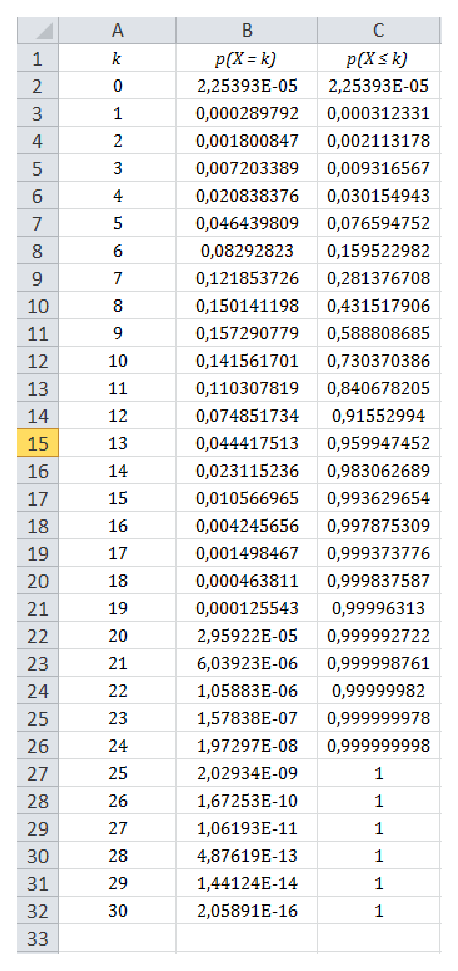
\includegraphics[width=0.9\linewidth]{echantillonnage.eps}\]
\end{minipage}\medskip

\begin{enumerate}[start=5]
    \item Recopier et compléter la phrase suivante :\par
    \textit{<< L'intervalle $\intervalleff{a}{b}$ est l'intervalle dans lequel la variable aléatoire $X$ prend ses valeurs avec une probabilité égale à environ... >>}
    
    \item Déterminer, pour $n = 30$, l'intervalle $\intervalleff{\frac a n}{\frac b n}$.\par
    Cet intervalle s'appelle \textit{intervalle de fluctuation d'une fréquence au seuil de $95\%$}.
\end{enumerate}

\end{document} 